% Copyright (c) 2014  Mirantis, Inc.
%
%    Licensed under the Apache License, Version 2.0 (the "License"); you may
%    not use this file except in compliance with the License. You may obtain
%    a copy of the License at
%
%         http://www.apache.org/licenses/LICENSE-2.0
%
%    Unless required by applicable law or agreed to in writing, software
%    distributed under the License is distributed on an "AS IS" BASIS, WITHOUT
%    WARRANTIES OR CONDITIONS OF ANY KIND, either express or implied. See the
%    License for the specific language governing permissions and limitations
%    under the License.
%
\documentclass[hyperref=unicode,utf8,xcolor=pst,aspectratio=169]{beamer}
\usetheme{boxes}
\setbeamertemplate{navigation symbols}{}
%
\definecolor{mirantisred}{RGB}{211,48,26}
\setbeamercolor{titlelike}{fg=mirantisred}
\setbeamercolor{structure}{fg=mirantisred}
\hypersetup{colorlinks,urlcolor=mirantisred}
%
\usepackage[T2A]{fontenc}
%
\usepackage{graphicx}
\usepackage{fancyvrb}
\usepackage{listings}
%
\newcounter{savedenum}
\newcommand*{\saveenum}{\setcounter{savedenum}{\theenumi}}
\newcommand*{\resume}{\setcounter{enumi}{\thesavedenum}}
%
\title{\fontsize{26}{0}\selectfont Ceph in Mirantis OpenStack}
\author{\vspace{-1mm}
\includegraphics[height=5cm]{Vector_RGB_MirantisLogo}\\Dmitry Borodaenko\vspace{-10mm}}
\date{Mountain View, 2014}
%
\begin{document}

\begin{frame}
	\titlepage
\end{frame}

\begin{frame}
	\frametitle{The Plan}
	\begin{columns}[T]
		\column{.55\textwidth}
		\begin{enumerate}
			\item What is Ceph?
			\item What is Mirantis OpenStack?
			\item How does Ceph fit with OpenStack?
			\item Where does Ceph not fit with OpenStack?
			\item What has Fuel got to do with Ceph?
			\item What does it look like?
			\item Things we do for Ceph in Fuel
			\item Things we do for Ceph in OpenStack
			\saveenum
		\end{enumerate}

		\column{.45\textwidth}
		\begin{enumerate}
			\resume
			\item Disk partitioning for Ceph OSD
			\item Cephx authentication settings
			\item Types of VM migrations
			\item Live VM migrations with Ceph
			\item Things we left undone
			\item Diagnostics
			\item Troubleshooting
			\item Resources
		\end{enumerate}
	\end{columns}
\end{frame}

\begin{frame}
	\frametitle{What is Ceph?}
	Ceph is a free distributed storage platform that provides unified
	object, block, and file storage.

	\begin{description}
		\item[Object Storage] Native RADOS objects: hash-based
			placement, synchronous replication;\\
			radosgw provides S3 and Swift compatible REST access to
			RGW objects (striped over multiple RADOS objects).
		\item[Block Storage] RBD block devices are thinly
			provisioned over RADOS objects and can be
			accessed by QEMU via librbd library.\\
			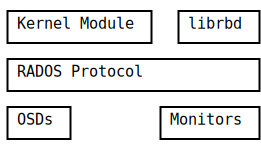
\includegraphics[height=2.5cm]{ceph-rbd}
		\item[File Storage] CephFS metadata servers (MDS)
			provide a POSIX-compliant file system backed by RADOS.
	\end{description}
\end{frame}

\begin{frame}
	\frametitle{What is Mirantis OpenStack?}
	\begin{columns}[T]
		\column{.5\textwidth}
		\begin{description}
			\item[OpenStack] is an open source cloud computing
				platform.
		\end{description}
		\column{.5\textwidth}
		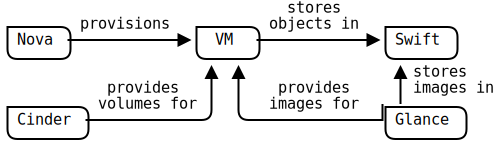
\includegraphics[height=2cm]{openstack-components}
	\end{columns}

	\begin{description}
		\item[Mirantis] ships hardened OpenStack packages and provides
			Fuel utility to automate deployment and lifecycle
			management of OpenStack environments.
	\end{description}

	\begin{columns}[T]
		\column{.43\textwidth}
		\begin{description}
			\item[Fuel] uses Cobbler, MCollective, and Puppet to
				discover nodes, provision OS, and setup
				OpenStack services.\\
		\end{description}
		\column{.65\textwidth}
		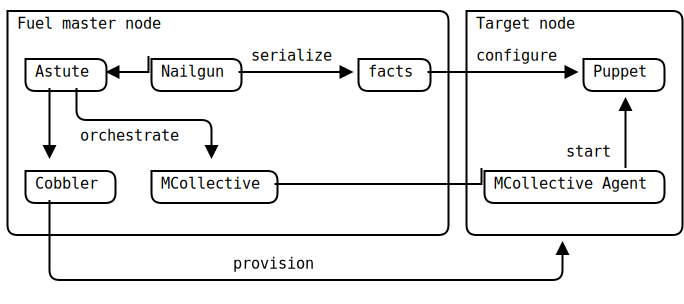
\includegraphics[height=3.8cm]{fuel-components}
	\end{columns}
\end{frame}

\begin{frame}
	\frametitle{How does Ceph fit with OpenStack?}
	\begin{columns}[T]
		\column{.6\textwidth}
		RBD drivers for OpenStack tell libvirt to configure the QEMU
		interface to librbd.

		\vspace{2ex}
		Ceph benefits:
		\begin{itemize}
			\item Multi-node striping and redundancy for block
				storage (Cinder volumes, Nova ephemeral drives,
				Glance images)
			\item Copy-on-write cloning of images to volumes and
				ephemeral disks, volumes to snapshots
			\item Unified pool of storage nodes for all types of
				data (objects, block devices, files)
			\item Live migration of Ceph-backed VMs
		\end{itemize}

		\column{.3\textwidth}
		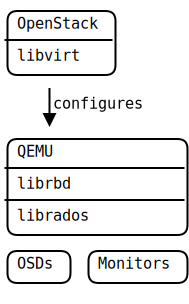
\includegraphics[height=6.5cm]{ceph-rbd-openstack}
	\end{columns}
\end{frame}

\begin{frame}
	\frametitle{Where does Ceph not fit with OpenStack?}
	\begin{itemize}
		\item RBD is not suitable for {\color{mirantisred}IOPS heavy
			workloads}:
			\begin{itemize}
				\item 100 IOPS per VM (HDD),
					10K IOPS per VM (SSD),
					10-100 ms latency
				\item high CPU load on OSD at high IOPS
					(each OSD needs 2 cores)
			\end{itemize}
		\item Low {\color{mirantisred}storage density}: requires
			erasure coding (preferrably combined with SSD-backed
			caching pools) to reduce replication factor below 3 for
			cold data
		\item {\color{mirantisred}Multi-site operation} options are
			limited:
			\begin{itemize}
				\item asynchronous replication is only
					implemented for radosgw and not for
					RBD
				\item master-slave mode is only useful for DR
					sites
				\item replication factor is multiplied by the
					number of sites
			\end{itemize}
		\item Ceph is sensitivite to {\color{mirantisred}clock drift}
			and {\color{mirantisred}network latency}
		\item {\color{mirantisred}Swift API} gaps in radosgw: bulk
			operations, custom account metadata, static website,
			expiring objects, object versioning, CORS
		\item Some code paths in OpenStack still do not work correctly
			with RBD:
			\begin{itemize}
				\item evacuate
				\item create image from volume
			\end{itemize}
	\end{itemize}
\end{frame}

\begin{frame}
	\frametitle{What has Fuel got to do with Ceph?}
	\begin{enumerate}
		\item Fuel deploys Ceph Monitors on controllers, and OSDs on
			dedicated nodes or in combination with OpenStack
			components.\\
			\includegraphics[height=3.7cm]{openstack-nodes}
			\vspace{-0.3cm}
		\item Creates XFS partitions for OSDs when provisioning
			ceph-osd nodes.
		\item Creates separate RADOS pools and sets up Cephx
			authentication for Cinder, Glance, and Nova.
		\item Configures Cinder, Glance, and Nova to use RBD backend
			with the right RADOS pools and Cephx credentials.
		\item Deploys radosgw behind HAProxy on controller nodes and
			registers it with Keystone.
	\end{enumerate}
\end{frame}

\begin{frame}
	\frametitle{What does it look like?}
	Select storage options $\Rightarrow$ Assign roles to nodes $\Rightarrow$ Allocate disks:\\
	\makebox[\textwidth][c]{\includegraphics[width=1.12\textwidth]{fuel-ceph-screenshots}}
\end{frame}

\begin{frame}
	\frametitle{Things we do for Ceph in Fuel}
	\begin{enumerate}
		\item Zap old partitions out of the way of ceph-disk (twice: in
			MCAgent on node delete, in pmanager during node
			provisioning)
		\item Set the right GPT Type GUIDs on OSD and journal
			partitions for Ceph's udev automount rules
		\item Set up root SSH between Ceph nodes for ceph-deploy
		\item Patch ceph-deploy to tolerate reordering of lines in
			ceph.conf
		\item Basic Ceph settings: cephx, pool size, networks
		\item List all Monitors in ceph.conf on each Ceph node
		\item Calculate initial PG numbers based on the number of OSDs
		\item radosgw: install Inktank's fork of FastCGI; set an
			infinite revocation interval for UUID auth tokens
		\item Live migrations for ephemeral backed VMs: disable SSH key
			injection; configure Nova, libvirt, and QEMU
	\end{enumerate}
\end{frame}

\begin{frame}
	\frametitle{Things we do for Ceph in OpenStack}
	Cinder patches:
	\begin{enumerate}
		\item Convert non-raw images when creating an
			RBD backed volume from Glance
	\end{enumerate}

	Nova patches:
	\begin{enumerate}
		\item Pass RBD user when invoking qemu-img CLI
		\item Use librbd instead of rbd CLI for most
			image operations
		\item Clone RBD backed Glance images into RBD
			backed ephemeral volumes
		\item Use Ceph cluster stats when reporting
			disk capacity for quotas
		\item Update VNC listen address on live migration
		\item Decouple shared block storage from shared libvirt
			instance path in the live migrations logic
		\item Decouple shared block storage in the evacuate logic
			(pending for Juno)
	\end{enumerate}
\end{frame}

\begin{frame}[fragile]
	\frametitle{Disk partitioning for Ceph OSD}
	Flow of disk partitioning information during discovery, configuration,
	provisioning, and deployment of ceph-osd nodes:\\
	\vspace{1ex}
	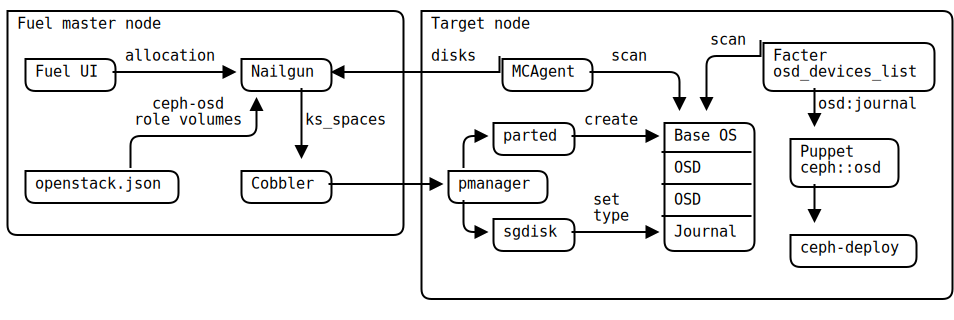
\includegraphics[height=3.7cm]{osd-disks}

	GPT partition type GUIDs according to ceph-disk:
	\lstset{language=Python,
		basicstyle=\ttfamily\footnotesize,
		keywordstyle=\color{blue}\ttfamily\footnotesize,
		stringstyle=\color{mirantisred}\ttfamily\footnotesize,
		commentstyle=\color{gray}\ttfamily\footnotesize
	}
	\begin{lstlisting}
	JOURNAL_UUID = '45b0969e-9b03-4f30-b4c6-b4b80ceff106'
	OSD_UUID     = '4fbd7e29-9d25-41b8-afd0-062c0ceff05d'
	\end{lstlisting}

	\vspace{1ex}
	If more than one device is allocated for OSD Journal, journal
	devices are evenly distributed between OSDs.
\end{frame}

\begin{frame}[fragile]
	\frametitle{Cephx authentication settings}
	\lstset{basicstyle=\ttfamily\footnotesize}

	Monitor ACL is the same for {\color{mirantisred}all} Cephx users:
	\vspace{-1ex}
	\begin{lstlisting}
	allow r
	\end{lstlisting}
	\vspace{1ex}

	OSD ACLs vary per OpenStack component:
	\vspace{-1ex}
	\begin{description}
		\item[Glance:]
			\begin{lstlisting}
			allow class-read object_prefix rbd_children,
			allow rwx pool=images
			\end{lstlisting}

		\vspace{-1.5ex}
		\item[Cinder:]
			\begin{lstlisting}
			allow class-read object_prefix rbd_children,
			allow rwx pool=volumes
			allow rx pool=images
			\end{lstlisting}

		\vspace{-1.5ex}
		\item[Nova:]
			\begin{lstlisting}
			allow class-read object_prefix rbd_children,
			allow rwx pool=volumes
			allow rx pool=images
			allow rwx pool=compute
			\end{lstlisting}
	\end{description}

	{\color{mirantisred}Watch out:} Cephx used to be easily tripped up by
	unexpected whitespace in ceph auth command line parameters, so we had
	to keep them all on a single line.
\end{frame}

\begin{frame}
	\frametitle{Types of VM migrations}
	{\bf OpenStack:}
	\begin{description}
		\item [Live vs offline:] Is VM stopped during migration?
		\item [Block vs shared storage vs volume-backed:] Is VM
			data shared between nodes? Is VM metadata
			(e.g. libvirt domain XML) shared?
	\end{description}

	{\bf Libvirt:}
	\begin{description}
		\item [Native vs tunneled:] Is VM state transferred
			directly between hypervisors or tunneled by
			libvirtd?
		\item [Direct vs peer-to-peer:] Is migration controlled
			by libvirt client or by source libvirtd?
		\item [Managed vs unmanaged:] Is migration controlled by
			libvirt or by hypervisor itself?
	\end{description}

	{\bf Our type:}\\
	Live, volume-backed*, native, peer-to-peer, managed.
\end{frame}

\begin{frame}
	\frametitle{Live VM migrations with Ceph}
	\begin{itemize}
		\item Enable native peer to peer live migration:\\
			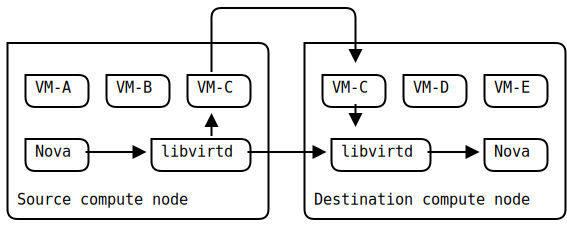
\includegraphics[height=3cm]{libvirt-p2p-migration}\\
			%libvirt flags: live, p2p, undefine-source, persist
			libvirt VIR\_MIGRATE\_* flags:\\
			LIVE, PEER2PEER, UNDEFINE\_SOURCE, PERSIST\_DEST
		\item Set VNC listen address to 0.0.0.0 and block VNC
			from outside the management network in iptables
		\item Open ports 49152+ between computes for QEMU
			migrations
	\end{itemize}
\end{frame}

\begin{frame}
	\frametitle{Things we left undone}
	\begin{enumerate}
		\item Ceph public network should go to a second storage
			network instead of management (blueprint:
			\href{https://blueprints.launchpad.net/fuel/+spec/fuel-storage-networks}{fuel-storage-networks})
		\item Dedicated Monitor and radosgw nodes (blueprint:
			\href{https://blueprints.launchpad.net/fuel/+spec/fuel-ceph-roles}{fuel-ceph-roles})
		\item Use clone\_image() when creating Glance images from
			Cinder volumes and Nova ephemeral disks, set more
			permissive Cephx ACLs across pools (bug: 
			\href{https://bugs.launchpad.net/fuel/+bug/1262914}{\#1262914})
		\item Multi-backend configuration for Cinder (blueprint:
			\href{https://blueprints.launchpad.net/fuel/+spec/fuel-cinder-multi-backend}{fuel-cinder-multi-backend})
		\item Replace ceph-deploy with direct use of Ceph CLI
	\end{enumerate}
\end{frame}

\begin{frame}[fragile]
	\frametitle{Diagnostics}
	\lstset{language=bash,basicstyle=\ttfamily\footnotesize}

	General health status of a Ceph cluster:
	\vspace{-2mm}
	\begin{lstlisting}
	ceph -s
	\end{lstlisting}

	Status of individual OSDs:
	\vspace{-2mm}
	\begin{lstlisting}
	ceph osd tree
	\end{lstlisting}

	Create empty Cinder volume:
	\vspace{-2mm}
	\begin{lstlisting}
	cinder create 1
	\end{lstlisting}

	Disk usage across all RADOS pools:
	\vspace{-2mm}
	\begin{lstlisting}
	rados df
	\end{lstlisting}

	Examine all RBD volumes in a single RADOS pool:
	\vspace{-2mm}
	\begin{lstlisting}
	rbd ls -l volumes
	\end{lstlisting}

	Upload a raw image to Glance, launch and live-migrate a VM:
	\vspace{-2mm}
	\begin{lstlisting}
	qemu-img convert -O raw cirros.qcow2 cirros.raw
	glance image-create --name cirros-raw --is-public yes \
	  --container-format bare --disk-format raw < cirros.raw
	nova boot --flavor 1 --image cirros-raw vm0
	nova live-migration vm0 node-3
	\end{lstlisting}
\end{frame}

\begin{frame}
	\frametitle{Troubleshooting}
	\begin{description}
		\item[disk partitioning failed during provisioning] --
			check if traces of previous partition tables are
			left on any drives
		\item['ceph-deploy osd activate' failed] -- same as above
		\item['ceph-deploy config pull' failed] -- check if the
			node can ssh to the primary controller over
			management network
		\item[HEALTH\_WARN: clock skew detected] -- check your
			ntpd settings, make sure your NTP server is
			reachable from all nodes
		\item[ENOSPC when storing small objects in RGW] -- try
			reducing rgw object stripe size
	\end{description}
\end{frame}

\begin{frame}
	\frametitle{Resources}
	Read the docs:\\
	\url{http://ceph.com/docs/master/rbd/rbd-openstack/}\\
	\url{http://docs.mirantis.com/fuel/fuel-5.1/}\\
	\url{http://libvirt.org/migration.html}

	\vspace{2ex}
	Get the code:\\
	\begin{itemize}
		\item \href{http://software.mirantis.com/}{Mirantis OpenStack} ISO image and VirtualBox scripts\\
		\item \href{https://github.com/stackforge/fuel-library/tree/master/deployment/puppet/ceph}{ceph} Puppet module for Fuel\\
		\item Nova branches: \href{https://github.com/jdurgin/nova/commits/havana-ephemeral-rbd}{havana-ephemeral-rbd},
			\href{https://github.com/angdraug/nova/commits/rbd-ephemeral-clone-stable-icehouse}{rbd-ephemeral-clone-stable-icehouse}
	\end{itemize}
\end{frame}

\end{document}
